\documentclass{beamer}
\usepackage{amsmath}
\usepackage{amssymb}
\usepackage{pgf}
\usepackage{tikz}
\usepackage{listings}
\usepackage{color}
\usetikzlibrary{matrix}
\usetheme{boxes}
\newcommand{\fig}{figures} % common figure path
\newcommand{\dbbslsh}{\textbackslash \textbackslash} % common figure path
\newcommand{\frnzplt}{FranzPlot }
\newenvironment{myblock}[3]{%
\definecolor{smtbx}{rgb}{0.64,0.76,0.68}
\setbeamercolor{block body}{#2}
\setbeamercolor{block title}{#3}
\begin{block}{#1}}{\end{block}}
\title[Curve e Sup. - Lab 3]{Curve e Superfici per il Design \\ Laboratorio 3 - Curve parametriche}
\author[Prof.ssa Scotti]{Prof.ssa Anna Scotti}
%\institute[dimat]{Long Inst.}
\date{7 Maggio 2019}

\begin{document}
%\lstset{language=POV}
\begin{frame}
\maketitle
\end{frame}
\section{Introduzione}
\begin{frame}
\frametitle{Materiali}
Nella cartella con il materiale di oggi troverete:
\begin{itemize}
\item Questa presentazione (\texttt{lab3.pdf})
\item Il file \texttt{screw\_bare.toml}.
\end{itemize}
Nella cartella `FranzPlot-DCS' troverete invece:
\begin{itemize}
%\item Il file \texttt{my\_include.inc}, che contiene delle macro (sequenze di comandi per povray) necessarie per fare alcuni esercizi.
\item L'eseguibile \texttt{franzplot.exe}
\end{itemize}
\end{frame}

%
\begin{frame}
\frametitle{Esercizio 1: Rette con \frnzplt - Il comando parametric curve}
Data la retta:
\begin{displaymath}
r:
\begin{cases}
x = t+2\\
y = -t+1\\
z = 2 t
\end{cases}
\end{displaymath}
\begin{itemize}
\item
Rappresentarla con \frnzplt attraverso l'elemento `parametric curve'.
\item Rappresentare inoltre un punto sulla retta.
\end{itemize}
\end{frame}
%
\begin{frame}
\frametitle{Esercizio 1b: Retta come traslazione di un punto}
\begin{enumerate}
\item Rimuovere dall'esercizio precedente la retta.
\item Traslare il punto scelto lungo la retta usando la trasformata temporale.
%\item Disegnare una retta combinando il punto scelto con una trasformazione spaziale di traslazione in funzione di un intervallo (input opzionale del nodo) opportunamente scelto, e mostrare che si ottiene la stessa retta del precedente esercizio
 \item Applicare, sempre allo stesso punto, un'operazione di traslazione
 spaziale lungo la direzione della retta, fissando come parametro della
 traslazione una variabile $u$ (e' possibile fissarla come input opzionale del
 nodo).
\item Sostituire la variabile $u$ con  un intervallo di valori (attraverso lo
stesso input opzionale) e mostrare che si ottiene la stessa retta.
\end{enumerate}
\end{frame}

%

%%
\begin{frame}
\frametitle{Esercizio 2: Filettatura di una vite}

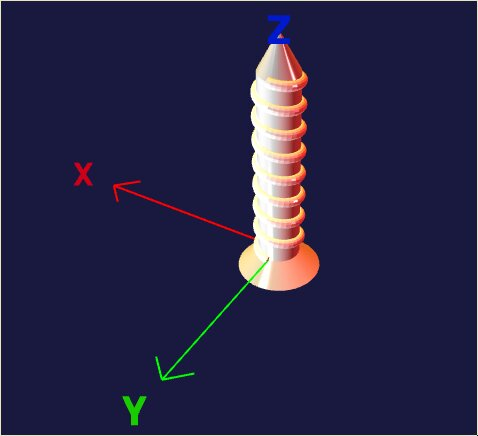
\includegraphics[width=0.5\textwidth]{\fig/screw_screwed.jpeg}

Determinare la curva parametrica che descrive la filettatura della vite in figura, a partire dal file \texttt{screw\_bare.toml}
\end{frame}
\begin{frame}
\frametitle{Esercizio 2-ii}
La curva \`e data dalla rotazione di un punto intorno all'asse composta con una traslazione lungo lo stesso asse, quindi si tratta di un'elica cilindrica.
\begin{displaymath}
\mathcal{C}:\begin{cases}
 x(t)= a\cos t\\
 y(t)=a \sin t\\
  z(t)= ct\qquad  0\leq t\leq 20\pi
\end{cases}
\end{displaymath}
Modificando i parametri $a$ e $c$ possiamo aggiustare raggio e passo dell'elica.
\end{frame}

%
\begin{frame}
\frametitle{Esercizio 3: Spirale conica}
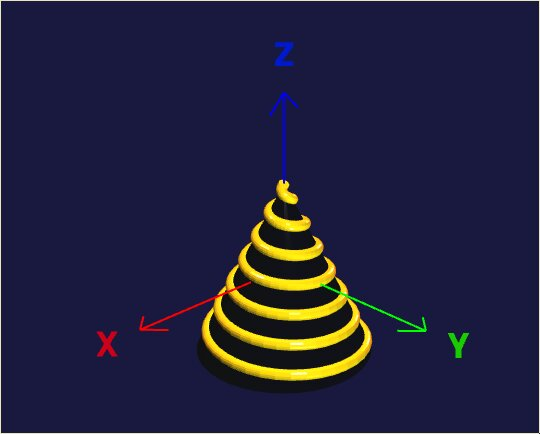
\includegraphics[width=0.5\textwidth]{\fig/cone_spiral.jpeg}\\
Determinare la curva parametrica che descrive il filo avvolto sul cono (da \texttt{primitive}). 
\end{frame}
\begin{frame}
\frametitle{Esercizio 3-ii}
La curva \`e data dalla rotazione di un punto intorno all'asse, con raggio
variabile, composta con una traslazione lungo lo stesso asse, quindi si tratta
di un'elica conica.  
\begin{displaymath}
\mathcal{C}:\begin{cases}
 x(t)= at\cos t\\
 y(t)=at \sin t\\
  z(t)= ct + d \qquad t_I\leq t\leq 0
\end{cases}
\end{displaymath}
Il rapporto fra $a$ e $c$ \`e legato alla semiapertura del cono. Usiamo valori
di $t$ negativi per disegnare il tratto inferiore dell'elica conica e $d$ per
traslare il vertice lungo $z$.  
\end{frame}
\begin{frame}
\frametitle{Esercizio 4: Sole/Terra/Luna}
L'equazione parametrica della circonferenza, ad esempio:
\begin{displaymath}
\mathcal{C}:\begin{cases}
 x(t)= a \cos t\\
 y(t)= a \sin t\\
 z(t)= 0
\end{cases}
\end{displaymath}
\`e utile anche per descrivere l'orbita dei corpi celesti. \\
Ponendo il sole al centro del sistema di riferimento, scrivere la curva che descrive il moto di un pianeta e di un suo satellite.\\
\begin{block}{Suggerimento}
Per ogni valore del parametro t, il moto del satellite rispetto al pianeta pu\`o essere visto come una rotazione
attorno al centro degli assi traslato della posizione del pianeta.  
\end{block}
\begin{itemize}
\item Rappresentare lo stesso sistema utilizzando punti e/o sfere ed il nodo \texttt{time transform}.
\end{itemize}
\end{frame}

\begin{frame}
\frametitle{Esercizio 4 - ii}

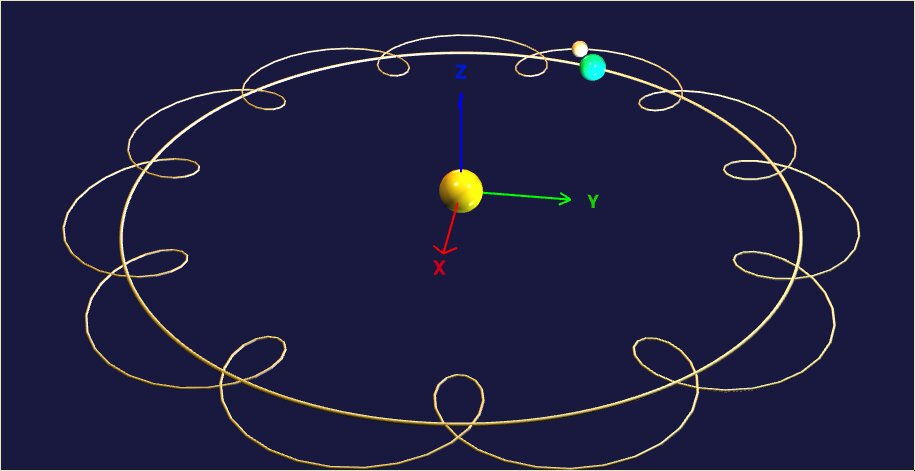
\includegraphics[width=0.8\textwidth]{\fig/sunsys.jpeg}
\\
Una curva come quella in figura \`e  qualitativamente l'unico tipo di curva osservabile?
\end{frame}


\begin{frame}
\frametitle{Esercizio 5}

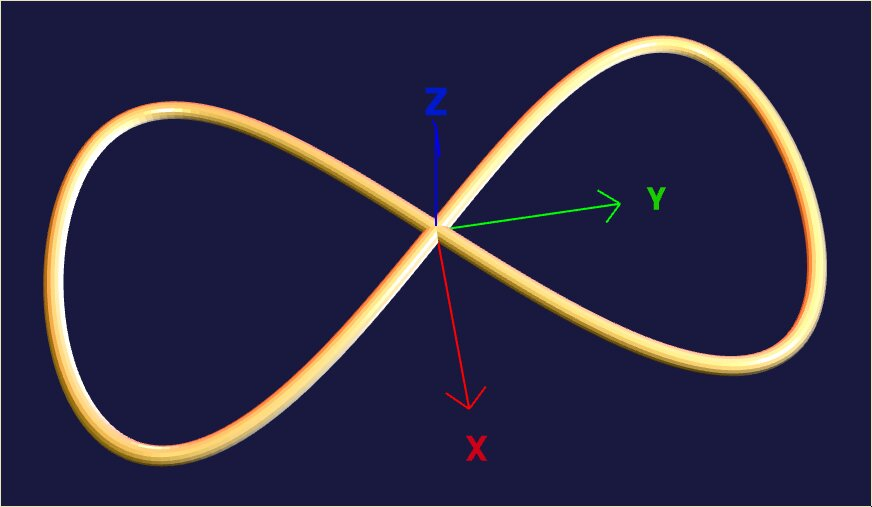
\includegraphics[width=0.8\textwidth]{\fig/infty.jpeg}

Determinare la forma della equazione parametrica che descrive questa curva. 
\end{frame}

\end{document}
